\section{Code}
github link: \url{https://github.com/nicoarrroyo/IPMLS/tree/main}

\section{IPDGS User Interface}
me when i'm an ipdgs user interface

\begin{figure}
     \centering
     \begin{subfigure}[b]{0.3\textwidth}
         \centering
         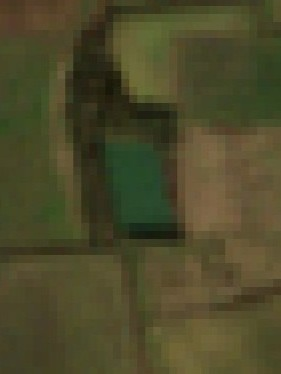
\includegraphics[width=\linewidth]{contents/figures/LR 10m res.jpg}
         \caption{User prompted on number of reservoirs}
         \label{fig:ipdgs ui first prompt}
     \end{subfigure}
     \hfill
     \begin{subfigure}[b]{0.3\textwidth}
         \centering
         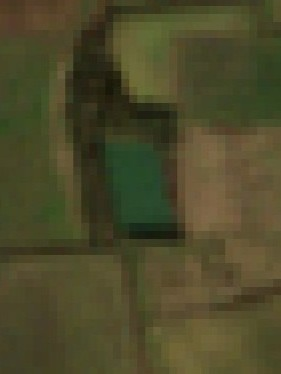
\includegraphics[width=\linewidth]{contents/figures/LR 10m res.jpg}
         \caption{User creating a polygon of the reservoirs' coordinates}
         \label{fig:ipdgs ui polygon}
     \end{subfigure}
     \hfill
     \begin{subfigure}[b]{0.3\textwidth}
         \centering
         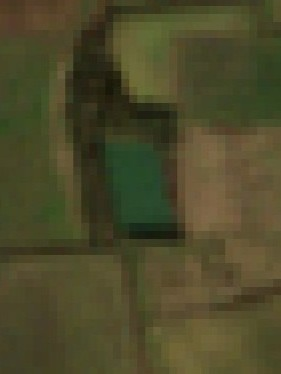
\includegraphics[width=\linewidth]{contents/figures/LR 10m res.jpg}
         \caption{IPDGS automatically generates the next chunk}
         \label{fig:ipdgs ui next chunk}
     \end{subfigure}
        \caption{Example IPDGS User Interface}
        \label{fig:ipdgs ui}
\end{figure}

